\documentclass[aspectratio=169]{beamer}
\usetheme{Madrid}
\usecolortheme{default}

% Packages
\usepackage{graphicx}
\usepackage{booktabs}
\usepackage{tikz}
\usetikzlibrary{shapes.geometric, arrows.meta, positioning, calc}

% Title Page
\title{Automated Bone Age Estimation Using Deep Learning}
\subtitle{Using Xception Architecture with Transfer Learning}
\author{
\textbf{Team Members:}\\[0.3cm]
Amit Anil Kamble (CS23B2034)\\
Jatin Goyal (CS23B2045)\\
Sumit Kumar (CS23B2008)\\[0.5cm]
\textbf{Guided By:}\\
Dr. Umarani Jayaraman\\
Assistant Professor
}
\institute{Pattern Recognition and Machine Learning Course}
\date{\today}

% Remove footers
\setbeamertemplate{footline}{}
\setbeamertemplate{navigation symbols}{}

\begin{document}

% Slide 1: Title
\frame{\titlepage}

% Slide 2: Problem Statement & Motivation
\begin{frame}{Problem Statement \& Motivation}
\begin{columns}
\column{0.5\textwidth}
\textbf{What is Bone Age Assessment?}
\begin{itemize}
    \item Evaluates skeletal maturity vs. chronological age
    \item Uses left hand X-ray comparison with atlas
    \item Critical for diagnosing growth disorders
\end{itemize}

\vspace{0.5cm}
\textbf{Why Automate?}
\begin{itemize}
    \item Manual method: time-consuming
    \item Inter-observer variability: $\pm6$-12 months
    \item Subjective judgment required
    \item Limited expert availability
\end{itemize}

\column{0.5\textwidth}
\begin{center}
\includegraphics[width=0.8\textwidth]{Fig7.png}
\end{center}
\end{columns}
\end{frame}

% Slide 3: Project Objectives
\begin{frame}{Project Objectives}
\begin{block}{Primary Goals}
\begin{itemize}
    \item Achieve R$^2$ score $\geq 0.92$ on validation data
    \item Maintain Mean Absolute Error (MAE) $\leq 12$ months
    \item Leverage transfer learning with Xception architecture
\end{itemize}
\end{block}

\begin{block}{Additional Analysis}
\begin{itemize}
    \item Gender-wise performance and bias analysis
    \item Developmental stage classification (Child/Adolescent/Adult)
    \item Model explainability via Grad-CAM visualization
\end{itemize}
\end{block}

\vspace{0.3cm}
\textbf{Dataset:} RSNA Pediatric Bone Age Challenge
\begin{itemize}
    \item 12,611 hand X-ray images with ground truth ages
    \item Age range: 1-228 months (0-19 years)
    \item Includes patient sex metadata
\end{itemize}
\end{frame}

% Slide 4: Methodology - Architecture
\begin{frame}{Model Architecture}
\begin{center}
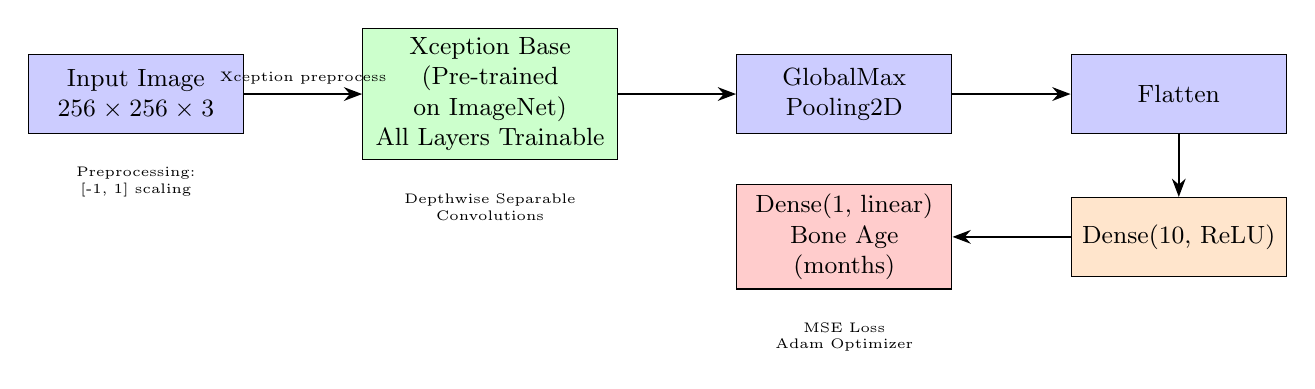
\begin{tikzpicture}[
    node distance=1.5cm,
    box/.style={rectangle, draw, fill=blue!20, text width=2.5cm, text centered, minimum height=1cm, font=\small},
    arrow/.style={-Stealth, thick}
]

% Input
\node[box] (input) {Input Image\\$256\times256\times3$};

% Xception Base
\node[box, fill=green!20, right=of input, text width=3cm] (xception) {Xception Base\\(Pre-trained on ImageNet)\\All Layers Trainable};

% Global Pooling
\node[box, right=of xception] (pool) {GlobalMax\\Pooling2D};

% Flatten
\node[box, right=of pool] (flatten) {Flatten};

% Dense Layer
\node[box, fill=orange!20, below=0.8cm of flatten] (dense) {Dense(10, ReLU)};

% Output
\node[box, fill=red!20, left=of dense, text width=2.5cm] (output) {Dense(1, linear)\\Bone Age\\(months)};

% Arrows
\draw[arrow] (input) -- node[above, font=\tiny] {Xception preprocess} (xception);
\draw[arrow] (xception) -- (pool);
\draw[arrow] (pool) -- (flatten);
\draw[arrow] (flatten) -- (dense);
\draw[arrow] (dense) -- (output);

% Labels
\node[below=0.3cm of input, font=\tiny, text width=2.5cm, align=center] {Preprocessing:\\ {[}-1, 1{]} scaling};
\node[below=0.3cm of xception, font=\tiny, text width=3cm, align=center] {Depthwise Separable\\Convolutions};
\node[below=0.3cm of output, font=\tiny, text width=2.5cm, align=center] {MSE Loss\\Adam Optimizer};

\end{tikzpicture}
\end{center}

\vspace{0.3cm}
\textbf{Key Configuration:} Batch Size=4, Epochs=50, LR=0.001, Early Stopping (patience=7)
\end{frame}

% Slide 5: Data Preprocessing & Augmentation
\begin{frame}{Data Preprocessing \& Augmentation}
\begin{columns}
\column{0.5\textwidth}
\textbf{Preprocessing Pipeline:}
\begin{enumerate}
    \item Resize to $256\times256$ pixels
    \item Apply \texttt{xception.preprocess\_input}
    \begin{itemize}
        \item Scales to $[-1, 1]$
        \item ImageNet mean/std normalization
    \end{itemize}
    \item No CLAHE or ROI cropping
\end{enumerate}

\vspace{0.5cm}
\textbf{Why Architecture-Specific?}
\begin{itemize}
    \item Generic rescaling ($1/255$) failed completely
    \item Xception expects specific input distribution
    \item Maintains transfer learning effectiveness
\end{itemize}

\column{0.5\textwidth}
\textbf{Data Augmentation:}
\begin{itemize}
    \item Horizontal flipping
    \item Rotation: $\pm10^\circ$
    \item Width/Height shift: $\pm10\%$
    \item Zoom: $\pm10\%$
    \item Fill mode: nearest
\end{itemize}

\vspace{0.5cm}
\textbf{Data Split:}
\begin{itemize}
    \item Training: $70\%$ (8,827 samples)
    \item Validation: $15\%$ (1,892 samples)
    \item Test: $15\%$ (1,892 samples)
    \item Stratified by age categories
\end{itemize}
\end{columns}
\end{frame}

% Slide 6: Approach Comparison
\begin{frame}{Approach Comparison: What We Tried}
\begin{table}
\centering
\small
\begin{tabular}{lccp{4cm}}
\toprule
\textbf{Approach} & \textbf{R² Score} & \textbf{MAE (months)} & \textbf{Notes} \\
\midrule
EfficientNet-B4 (frozen) & 0.70 & 33 & Frozen layers, wrong preprocessing \\
Xception + CLAHE & -0.01 & N/A & CLAHE destroyed performance \\
Xception + ROI crop & 0.68 & 28 & Lost important edge information \\
\rowcolor{green!20}
\textbf{Our Final Model} & \textbf{0.9169} & \textbf{9.04} & \textbf{All layers trainable} \\
Kaggle Best & $\sim$0.95 & $\sim$8-10 & Heavy hyperparameter tuning \\
\bottomrule
\end{tabular}
\end{table}

\vspace{0.5cm}
\begin{block}{Key Insights}
\begin{itemize}
    \item Architecture-specific preprocessing is \textbf{critical} for transfer learning success
    \item Training all layers from start outperforms gradual unfreezing
    \item Contrast enhancement (CLAHE) breaks transfer learning from ImageNet
    \item Simple regression heads (10 units) work well with strong base models
\end{itemize}
\end{block}
\end{frame}

% Slide 7: Results - Regression Performance
\begin{frame}{Results: Regression Performance}
\begin{columns}
\column{0.4\textwidth}
\textbf{Validation Metrics:}
\begin{table}
\small
\begin{tabular}{lc}
\toprule
\textbf{Metric} & \textbf{Value} \\
\midrule
R² Score & \textcolor{blue}{\textbf{0.9169}} \\
MAE & \textcolor{blue}{\textbf{9.04 mo}} \\
RMSE & 11.75 mo \\
Within ±12mo & 91.5\% \\
\bottomrule
\end{tabular}
\end{table}

\vspace{0.3cm}
\begin{block}{Target Achievement}
$\checkmark$ R$^2$ = 0.9169 (target: $\geq 0.92$)\\
$\checkmark$ MAE = 9.04 mo (target: $\leq 12$ mo)\\
\textcolor{green}{\textbf{Objectives Met!}}
\end{block}

\column{0.6\textwidth}
\begin{center}
\includegraphics[width=\textwidth]{Fig1.png}
\end{center}
\end{columns}
\end{frame}

% Slide 8: Results - Training & Error Analysis
\begin{frame}{Training History \& Error Analysis}
\begin{columns}
\column{0.5\textwidth}
\textbf{Training Curves:}
\begin{center}
\includegraphics[width=\textwidth]{Fig3.png}
\end{center}
\begin{itemize}
    \item Converged at epoch 18
    \item Early stopping prevented overfitting
    \item Stable validation performance
\end{itemize}

\column{0.5\textwidth}
\textbf{Residual Plot:}
\begin{center}
\includegraphics[width=\textwidth]{Fig2.png}
\end{center}
\begin{itemize}
    \item Errors centered around zero
    \item Most predictions within $\pm12$ months
    \item Slight heteroscedasticity at extremes
\end{itemize}
\end{columns}
\end{frame}

% Slide 9: Gender Bias Analysis
\begin{frame}{Gender Bias Analysis}
\begin{columns}
\column{0.4\textwidth}
\textbf{Performance by Gender:}
\begin{itemize}
    \item Male samples: Similar performance
    \item Female samples: Similar performance
    \item MAE difference: $< 2$ months
    \item R$^2$ difference: $< 0.01$
\end{itemize}

\vspace{0.5cm}
\begin{block}{Bias Assessment}
\textcolor{green}{\textbf{$\checkmark$ Low Bias Detected}}\\
MAE difference less than 2 months between genders is clinically acceptable.\\
\textbf{Fair predictions across both genders.}
\end{block}

\column{0.6\textwidth}
\begin{center}
\includegraphics[width=\textwidth]{Fig4.png}
\end{center}
\end{columns}
\end{frame}

% Slide 10: Classification & Explainability
\begin{frame}{Classification \& Model Explainability}
\begin{columns}
\column{0.5\textwidth}
\textbf{Developmental Stage Classification:}
\begin{center}
\includegraphics[width=0.9\textwidth]{Fig5.png}
\end{center}
\begin{itemize}
    \item Overall Accuracy: \textbf{91.54\%}
    \item QWK: \textbf{0.8248}
    \item Child (0-10y): 95\% recall
    \item Adolescent (10-18y): 91\% recall
\end{itemize}

\column{0.5\textwidth}
\textbf{Grad-CAM Visualization:}
\begin{center}
\includegraphics[width=0.7\textwidth]{Fig6.png}
\end{center}
\begin{itemize}
    \item Shows model attention regions
    \item Focuses on carpal bones \& growth plates
    \item Red/Yellow = High importance
    \item Blue/Purple = Low importance
    \item \textbf{Model is interpretable \& trustworthy}
\end{itemize}
\end{columns}
\end{frame}

% Slide 11: Key Findings & Challenges
\begin{frame}{Key Findings \& Challenges}
\begin{columns}
\column{0.5\textwidth}
\textbf{What Worked Well:}
\begin{enumerate}
    \item \textbf{Xception's preprocessing}\\
    Architecture-specific preprocessing was game-changer
    
    \item \textbf{Training all layers}\\
    Training from epoch 1 outperformed gradual unfreezing
    
    \item \textbf{Simple regression head}\\
    Just 10 dense units avoided overfitting
    
    \item \textbf{Transfer learning}\\
    ImageNet pre-training provided excellent features
\end{enumerate}

\column{0.5\textwidth}
\textbf{Challenges Encountered:}
\begin{enumerate}
    \item \textbf{GPU memory constraints}\\
    Limited to batch size=4 on RTX 3060 12GB
    
    \item \textbf{Preprocessing experimentation}\\
    Multiple failed attempts before finding correct approach
    
    \item \textbf{Class imbalance}\\
    Fewer samples at age extremes affected performance
    
    \item \textbf{Computation time}\\
    Training took 2-3 hours with mixed precision
\end{enumerate}
\end{columns}
\end{frame}

% Slide 12: Conclusion & Future Work
\begin{frame}{Conclusion \& Future Work}
\begin{block}{Summary}
We successfully developed an automated bone age estimation system achieving:
\begin{itemize}
    \item \textbf{R$^2$ = 0.9169, MAE = 9.04 months} (meeting project objectives)
    \item \textbf{Low gender bias} ensuring fair predictions
    \item \textbf{91.54\% classification accuracy} for developmental stages
    \item \textbf{Model explainability} through Grad-CAM visualization
\end{itemize}
\end{block}

\begin{columns}
\column{0.5\textwidth}
\textbf{Limitations:}
\begin{itemize}
    \item Dataset primarily Caucasian patients
    \item Single modality (hand X-rays only)
    \item No uncertainty estimation
    \item Clinical validation needed
\end{itemize}

\column{0.5\textwidth}
\textbf{Future Work:}
\begin{itemize}
    \item Multi-ethnic dataset validation
    \item Incorporate patient metadata (gender, height)
    \item Uncertainty quantification
    \item Integration with PACS systems
    \item Prospective clinical trials
\end{itemize}
\end{columns}

\vspace{0.5cm}
\centering
\Large{\textbf{Thank You! Questions?}}
\end{frame}

\end{document}
